% Copyright (C) 2010,2011,2012,2013,2014,2015,2016 The ESPResSo project
% Copyright (C) 2002,2003,2004,2005,2006,2007,2008,2009,2010 
%   Max-Planck-Institute for Polymer Research, Theory Group
%  
% This file is part of ESPResSo.
%   
% ESPResSo is free software: you can redistribute it and/or modify it
% under the terms of the GNU General Public License as published by the
% Free Software Foundation, either version 3 of the License, or (at your
% option) any later version.
%  
% ESPResSo is distributed in the hope that it will be useful, but
% WITHOUT ANY WARRANTY; without even the implied warranty of
% MERCHANTABILITY or FITNESS FOR A PARTICULAR PURPOSE.  See the GNU
% General Public License for more details.
%  
% You should have received a copy of the GNU General Public License
% along with this program.  If not, see <http://www.gnu.org/licenses/>.
%
%%%%%%%%%%%%%%%%%%%%%%%%%%%%%%%%%%%%%%%%%%%%%%%%%%%%%%%%%%%%%%%%% 
% From the brainstorming:
%
% Preknowledge:
% 
% Basic MD(simple integrator,langevin thermostat, ---basic tcl
% basic potentials, basis tutorial 1
% 
% Basis Tutorial: written in Latex
% 
% <<every line of script code should be explained>>
% 
% 1) tcl basic setting up a system
% MD, soft sphere and Lennard-Jones Fluid (argon system), 
% Units
% 
% online visualization (pdb output)
% rdf, pressure,energy,
% 
% online analysis function
% savin, readin writeout, offline analysis, statistics
% 
% Structure:
% Part1:
% 1) Prerequisits (what you should know beforehand: basic tcl knowledge,
% Here you can find more info: Allen, Tildesley: Frenkel smit,
% Rappaport, tcl tutorial,
% 
% 2) Physics of the systems (argon, soft sphere system)
% 
% 3) Algorithms (verlocity verlet, Langevin, Potentials, LJ)
% 3b) about units
% 
% Part2 
% 1) simulation script in all detail, line by line
% Initialize
% Visualize
% Simulate (with online analysis, saves for later off-line analysis,
% (Savelize (save our lives ))
% 
% 2) a new script for later
% analysis, and other helper ideas
% 
% Things to remember and take care of:
% Use the same names for variables
% 
% ====================================================================
% General Tutorial: (the next tutorials: pe_solution, cell model of one
% charged colloid, LB, ferrofluid)
% 
\documentclass[
paper=a4,                       % paper size
fontsize=11pt,                  % font size
twoside,                        % two sided
footsepline,                    % add a line to separate the footer
headsepline,                    % add a line to separate the header
headinclude=false,              % header does not belong to the text
footinclude=false,              % footer does not belong to the text
pagesize,                       % set the pagesize in a DVI document
]{scrartcl}

% Do magic that \bfseries for keywords actually works
\DeclareFontShape{OT1}{cmtt}{bx}{n}{<5><6><7><8><9><10><10.95><12><14.4><17.28><20.74><24.88>cmttb10}{}

% Custom colors
\definecolor{stringblue}{rgb}{0.09,0.211,0.57}
\definecolor{codered}{rgb}{0.655,0.1137,0.3747}
\definecolor{deepgreen}{rgb}{0,0.5,0}
\definecolor{commentgray}{rgb}{0.4,0.4,0.4}
\definecolor{framegray}{rgb}{0.8,0.8,0.8}
\lstdefinestyle{pypressostyle}{
  language=Python,
  belowcaptionskip=1\baselineskip,
  breaklines=true,
  xleftmargin=\parindent,
  showstringspaces=false,
  stringstyle=\color{orange},
  belowskip=\bigskipamount,
  aboveskip=\bigskipamount,
  basicstyle=\ttfamily\small,
  otherkeywords={self},             % Add keywords here
  keywordstyle=\bfseries\color{codered},
  moredelim=*[s][]{.}{\ },
  moredelim=*[s][]{\ }{.},
  moredelim=*[s][]{.}{\[},
  emph={accuracy,
        actors,
        Actors,
        Actor,
        add,
        add_bond,
        Analysis,
        analyze,
        Angle_Cosine,
        Angle_Cossquare,
        Angle_Harmonic,
        bjerrum_length,
        BondedInteraction,
        BondedInteractionNotDefined,
        BondedInteractions,
        bonded_inter,
        bonded_interaction_classes,
        box_l,
        cellsystem,
        CellSystem,
        code_info,
        COORDS_ALL_FIXED,
        COORDS_FIX_MASK,
        COORD_FIXED,
        cuda_init,
        CudaInitHandle,
        cutoff,
        Dihedral,
        electrostatics,
        Endangledist,
        epsilon, 
        espressomd,
        features,
        FeneBond,
        galilei,
        GalileiTransform,
        harmonic,
        HarmonicBond,
        HarmonicDumbbellBond,
        highlander,
        id,
        integrate,
        integrator,
        Integrator,
        interactions,
        lennard_jones,
        minimize_energy,
        MinimizeEnergy,
        non_bonded_inter, 
        NonBondedInteraction,
        NonBondedInteractionHandle,
        NonBondedInteractions,
        Oif_Global_Forces,
        Oif_Local_Forces,
        OrderedDict,
        Overlapped,
        part,
        particle_data,
        PARTICLE_EXT_FORCE,
        PARTICLE_EXT_TORQUE,
        ParticleHandle,
        ParticleList,
        ParticleSlice,
        polymer,
        Polymer,
        pos,
        P3M,
        q,
        RigidBond,
        run,
        set_params,
        set_steepest_descent,
        shift,
        sigma,
        steps,
        System,
        Tabulated,
        ThereCanOnlyBeOne,
        thermostat,
        Thermostat,
        time_step,
        update_wrapper,
        utils,
        v,
        Virtual},          % Custom highlighting
  emphstyle=\bfseries\color{deepgreen},    % Custom highlighting style
  commentstyle=\color{commentgray}\ttfamily,
  stringstyle=\color{stringblue},
  frame=tb,                         % Any extra options here
  rulecolor=\color{framegray},
  showstringspaces=false            % 
}
\lstnewenvironment{pypresso}{%
  \lstset{style=pypressostyle}}{}


%% Grafikpakete
\usepackage{graphicx}%


\usepackage{verbatim}

% How to diplay ESPResSo commands in flowing text. Larger code segments
% should be put inside boxes.
\newcommand{\EScmd}[1]{\texttt{\textbf{#1}}}

% The code block
%\newcommand{\EScode}[1]{ \parbox{0.95\textwidth}{\texttt{#1}}}
\usepackage{listings} 
\lstset{numbers=left, numberstyle=\tiny, numbersep=5pt, showspaces=false, showstringspaces=false,postbreak=\space, breakindent=5pt, breaklines}
\lstset{language=tcl, keywordstyle=\color{blue}\bfseries ,emphstyle=\color{green}, commentstyle=\color{red}\itshape }
\lstset{keywordsprefix=setmd}
\lstset{keywords=[6]{thermostat,part,inter,integrate,rescale_velocities,code_info,save_sim,writepdb,analyze,uwerr}}

\newtheorem{task}{Task}

\begin{document}

\esptitlehead

\title{Tutorial 1: Lennard-Jones Liquid%
\ifdefined\esversion%
\thanks{For \es \esversion}%
\fi%
}
\subtitle{\es Basics}
\author{H.-J. Limbach \and M. S\"uzen \and K. Grass \and M. Sega \and
  A. Arnold \and N. Gribova}
\maketitle
\tableofcontents

\section{Introduction}

Welcome to the basic \es{} tutorial!

In this tutorial, you will learn, how to use the \es{} package for your 
research. We will cover the basics of \es, i.e.~how to set up and modify a 
physical system, how to run a simulation, and how to load, save and analyze the 
data.

The more advanced features and algorithms available in the \es{} package will 
be described in additional tutorials in the future.

\section{Background}
Today's research on Soft Condensed Matter has brought the needs for having a 
flexible, extensible, reliable and efficient (parallel) molecular simulation 
package. For this reason \es{} (Extensible Simulation Package for Research on 
Soft matter) \cite{esp_url} has been developed in Max Planck Institute for 
Polymer Research, Mainz by the Group of PD Dr. Christian Holm 
\cite{limbach2006ees}. The Espresso package is probably the most flexible and 
extensible simulation package in the market. It is specially developed for 
coarse-grained molecular dynamics (MD) simulation of polyelectrolytes but not 
necessarily limited to this. It can be used even in simulating granular media 
for example. \es{} has been nominated for the Heinz-Billing-Preis for 
Scientific Computing in 2003 \cite{arnold2003ees}.

\section{Tutorial Outline}

% 1) Prerequisits
% 
% 2) Physics of the systems
% 
% 3) Simulation setup and details
% 
% 4) Analysis
% 
% 5) Outlook: what else you can do with this system

In this short tutorial, you will be introduced to the \es{} package as smooth 
as possible with a minimal set of skills. We will guide you through the initial 
steps of working with \es{} and help you to examine a simple physical system, a 
Lennard-Jones liquid.

After a brief introduction to \es{} in Section \ref{sec:espresso}, we provide 
you with a short tutorial to the Tcl programming language which is used to 
control simulations using \es{} in Section \ref{sec:tcl}. In Section \ref{sec:ljliquid}, we will 
introduce you to the problem system studied in this tutorial and familiarize you with the necessary 
background knowledge. Please note, however, that it is beyond the scope of this 
tutorial to give a complete overview of the the area. We give a few 
references that can give you more detailed information regarding MD.

%In Section \ref{sec:vmd}, we demonstrate how to visualize simulation data with 
%\emph{VMD\footnote{\texttt{http://www.ks.uiuc.edu/Research/vmd/}}} and how to 
%analyze it with the aid of the functions provided by \es{}. At the end of this tutorial,
%you will be able to compare your results to the ones obtained in the original 
%investigations on the presented topic.

%We conclude this basic tutorial with an outlook on the more advanced features 
%of \es{} that will be detailed in future tutorials.

%%%%%%%%%%%%%%%%%%%%%
%%%%%%%%%%%%%%%%%%%%%
%%%%%%%%%%%%%%%%%%%%%
\section{First steps}\label{sec:espresso}

  What is \es{}? It is not a coffee, indeed. It is an extensible, efficient 
  Molecular Dynamics package specially powerful on simulating charged systems. 
  In depth information about the package can be found in the relevant sources 
  \cite{esp_url,arnold2003ees} and a recent paper \cite{limbach2006ees}.

  From the users point of view, \es{} is driven by Tcl(/TK)\footnote{Tool
  command language} \cite{tcl_url}, that the
  user can interact with the package core via command line interface (CLI) or 
  scripts by using Tcl scripting language\footnote{In short, a \emph{scripting language
  } allows the user to write instructions that are carried out by an interpreter
  without prior compiling. This enables the user to use \es{} for vastly
  different applications without the need of different specialized executable files.}.
  In a given \es{} script, some commands
  are interpreted by the scripting language (Tcl), while others by the core
  \es{} program written in C. However, all \es{} commands and directives in the
  script are
  transparent to the user, regardless of its implementation either on the C- or Tcl-level.

\emph{Note: This tutorial assumes that you already have a working \es{}
installation on your system. If this is not the case, please go to
\texttt{http://espressomd.org/} for information on how to obtain and
install \es{}.}

\vspace{1cm}\framebox{\begin{minipage}{0.95\textwidth} 
         \begin{task} 
             To start \es{}, simply type \texttt{Espresso} in the command 
             line shell. This will open the Command Line Interface (CLI) of
             \es{}. Upon issuing the \es{} command
             \lstinline|code_info| you can see the options that are included in 
             your \es{} binary\footnote{\es{} provides many different features,
             some which are mutually exclusive. This is why not all features are
             activated by default, but instead have to be explicitly requested
             at compile time of the executable. Please consult the user's guide
             for details on this.}.

\end{task}
\end{minipage}}\vspace{1cm}

%\usepackage{graphics} is needed for \includegraphics
\begin{figure}[htp]
\begin{center}
  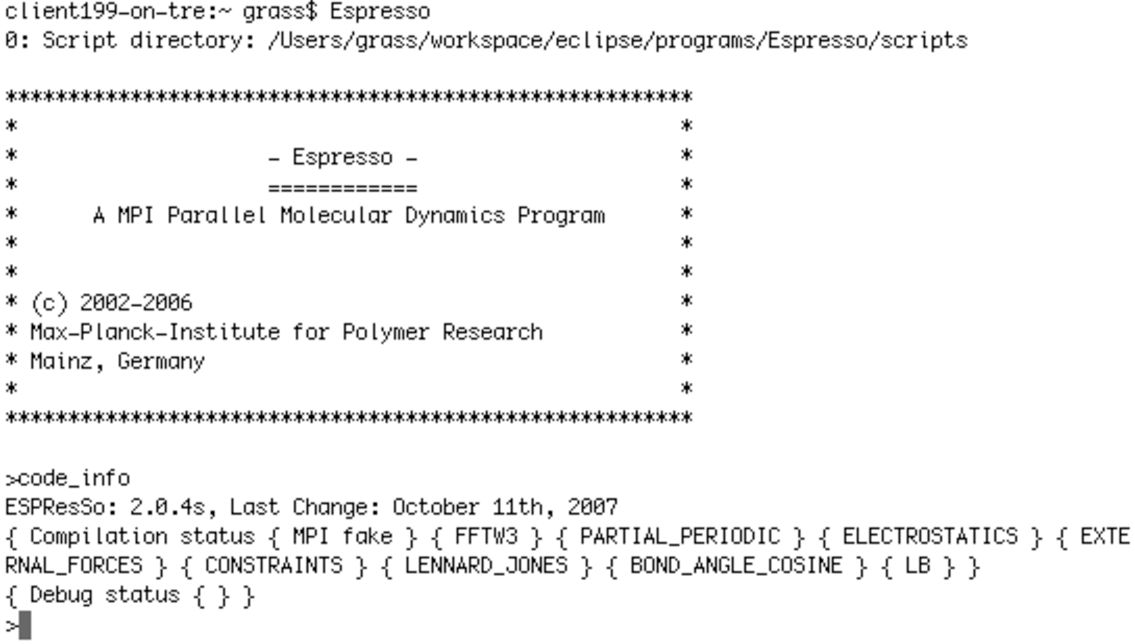
\includegraphics[width=0.95\textwidth]{figures/espresso-output.pdf}
  \caption{Example output of the \es{} Command Line Interface upon issuing the
  \lstinline|code_info| command.}
  \label{fig:espresso_output}
\end{center}
\end{figure}

\vspace{1cm}\framebox{\begin{minipage}{0.95\textwidth} 
         \begin{task} 
  
  Figure \ref{fig:espresso_output} shows the
             terminal output you should have obtained. What kind of output
             are you receiving from  \lstinline|code_info| command?
\end{task}
\end{minipage}}\vspace{1cm}

On the screenshot you can see several compiled in features, i.e.~the fake multiprocessing interface, the fast Fourier transform, the Lennard-Jones and electrostatic potential. All features can be found explained in the \es{} User Guide.

%%%%%%%%%%%%%%%%%%%%%
%%%%%%%%%%%%%%%%%%%%%
%%%%%%%%%%%%%%%%%%%%%
 \section{Short TCL Tutorial}\label{sec:tcl}

   Tcl (Tool Command Language) is a very powerful but easy to learn programming
   language. \footnote{It is dynamically interpreted, which means that commands are read,
   interpreted, and executed by the computer one command line at a time.} 
   Aside from writing any valid Tcl code, the user can write any valid \es{}
   command on the \es{} CLI. Here we will review the 
   basic Tcl tutorial \cite{tcl_tut_url} in Espresso CLI. Now type 
   \texttt{Espresso}. Once in the CLI, you can familiarize yourself with the 
   basics of TCL. 
   
    \subsection{Assignments and evaluation}
     A simple text output, or a print statement can be carried out with 
     \lstinline|puts| \footnote{Valid TCL / \es{} commands are bold and blue, all following code can be direct used with \es{}.}
      

{\vspace{0,2cm}\small
\begin{lstlisting}[numbers=none]
puts "Hello Espresso \n"
puts "This is line 1"; puts "this is line 2"
\end{lstlisting}\vspace{0,2cm}
}

\noindent In order to declare a variable and/or assign a value to it, you use the
assignment command, called \lstinline|set|.

{\small\vspace{0,2cm}
\begin{lstlisting}[numbers=none]
set X "This is a string"
set Y 1.24
puts $X
puts $Y
\end{lstlisting}\vspace{0,2cm}
} 

\noindent When assigning a value to a variable, the variable is accessed simply by its
variable name (as in the first line, \texttt{X}). When a value is accessed, the variable
name is preceded by a dollar sign (as in the third line, \texttt{\$X})

\noindent C-like backslash sequences can be used along \lstinline|put|. For example,
\texttt{\textbackslash{}t} puts a tab, \texttt{\textbackslash{}r} puts a line return and \texttt{\textbackslash{}n} puts a carriage
return. Comments are placed using a hash (\#) sign.

{\small\vspace{0,2cm}
\begin{lstlisting}[numbers=none]
set X 1.2 ;	# this is a comment
set Y 2.1 ;	# another comment
puts "\t tab \t another tab \n X=$X and Y=$Y "
\end{lstlisting}\vspace{0,2cm}
} 

\noindent To evaluate the result of mathematical expressions you can use the 
\lstinline|expr| command. Note, that the entire statement is enclosed in square brackets. 

{\small\vspace{0,2cm}
\begin{lstlisting}[numbers=none]
set X  60
set Y  30
set Z [expr $X+$Y]
puts " X=$X and Y=$Y and X+Y=$Z"
set cosX [expr cos($X)]
puts "cos ($X) =  $cosX"
\end{lstlisting}\vspace{0,2cm}
}

\noindent Most C-like operators and math functions are valid TCL syntax.

\subsection{Comparisons and looping}

Syntax of numeric comparison is as follows 

{\small\vspace{0,2cm}
\begin{lstlisting}[numbers=none]
set x 5
if {$x == 5} {puts "$x is 5"} else {puts "$x is not 5"}
\end{lstlisting}\vspace{0,2cm}
} 
      
\noindent You may also write this in different lines by using backslashes. As in
many shell scripting languages such as Tcl, the  backslash is
used for line continuation only in the Espresso CLI, not when running a loaded script.
However, there is one exception: even in a script, Tcl expects all parameters of a function,
including flow control commands such as \texttt{if} or \texttt{while}, on the same line. Here
you need continuation backslashes even in a script. However, a block with in curled braces,\
which is the most common in Tcl, does not require backslashes for continuation inside. Therefore,
in a script, the above code might look like this:
{\small\vspace{0,2cm}
\begin{lstlisting}[numbers=none]
set x 5
if {$x == 5} {
  puts "$x is 5"
} else {
  puts "$x is not 5"
}
\end{lstlisting}\vspace{0,2cm}
}
\noindent but still, you need the backslashes in this style:
{\small\vspace{0,2cm}
\begin{lstlisting}[numbers=none]
set x 5
if {$x == 5} \
  { puts "$x is 5" } \
else \
  { puts "$x is not 5" }
\end{lstlisting}\vspace{0,2cm}
}

You can loop with standard \lstinline|for| or \lstinline|while| constructs. 
For example finding $10!$ with the \lstinline|for| construct:
      
{\small\vspace{0,2cm}
\begin{lstlisting}[numbers=none]
set factorial 1.0
for {set i 1} {$i <11} {incr i} \
  {set factorial [expr $factorial*$i]}
puts "10! is $factorial"
\end{lstlisting}\vspace{0,2cm}
}

\noindent Or with a  \lstinline|while| construct

{\small\vspace{0,2cm}
\begin{lstlisting}[numbers=none]
set factorial 1.0
set i 1
while {$i <11} {set factorial [expr $factorial*$i] ; incr i}
puts "10! is $factorial"
\end{lstlisting}\vspace{0,2cm}
 }
 
 \subsection{Lists}
 
 An ordered collection of entities can be assigned to a variable that 
 makes it a \lstinline|list|\footnote{This is similar - but not entirely equivalent - to
 arrays in computer languages such as C or C++.}. This is the basic data
 structure in TCL. Lists can be set similar to variables.
 To access the list data one can use \lstinline|lindex| by using corresponding 
 index value. Remember that in TCL the list indices start with 0 like in other scripting/programming languages .
 
 {\small\vspace{0,2cm}
\begin{lstlisting}[numbers=none]
set x "1 2 3"
puts "first element is [lindex $x 0]"
puts "second element is [lindex $x 1]"
puts "and the last [lindex $x 2]"
\end{lstlisting}\vspace{0,2cm}
}

\noindent One can access all the elements by using \lstinline|foreach| looping 
construct as well

{\small\vspace{0,2cm}
\begin{lstlisting}[numbers=none]
set i 0
foreach  j $x {\
  puts "$j is item number $i in list x"; incr i}
\end{lstlisting}\vspace{0,2cm}
}

\noindent Also we can access list of lists

{\small\vspace{0,2cm}
\begin{lstlisting}[numbers=none]
set y "{l00 l01} {l10 l11} {l20 l21}"
puts "first element of second list is [lindex $y 1 0]"
puts "second element of third list is [lindex $y 2 1]"
\end{lstlisting}\vspace{0,2cm}
}

\noindent We can also find the length of a list by \lstinline|llength|, append an 
element by \lstinline|lappend| and inserting an element by \lstinline|linsert|:
       
{\small\vspace{0,2cm}
\begin{lstlisting}[numbers=none]
set x "1 2 3 4" ; 	# generate a list x
llength $x ;		# get the size of list x (number of elements)
lappend x 5 ;		# add a new member end of list
puts "x is {$x}" ;		# print list again
set x [linsert $x 3 3a] ;	# insert an element "3a" at index 3
puts "x is {$x}" ;		# print list again
\end{lstlisting}
}\vspace{0,2cm}

\section{Adding a new Tcl command}
     
In Tcl there is actually no distinction between commands (often known as 
'functions' in other languages) and "syntax" \cite{tcl_tut_url}

{\small\vspace{0,2cm}
\begin{lstlisting}[numbers=none]
proc sum {arg1 arg2}  { \
set x [expr {$arg1 + $arg2}]; \
return $x \
} 
sum  1 4
puts [sum 1 4]

\end{lstlisting}\vspace{0,2cm}
}


\subsection{Writing to a file}
It is useful to write the data into a file. For example

{\small\vspace{0,2cm}
\begin{lstlisting}[numbers=none]
set file_handle [open "file.dat" "w"];
		# open a file called file.dat to write 
		# and file channel is $file_handle
		
puts $file_handle "This will go into file!"
for {set i 0} {$i <10} {incr i} { \
   puts $file_handle "counting $i"  }

close $file_handle ;			# close file channel
set file_content [exec cat file.dat] ;
					# exec runs shell commands
puts "$file_content"
exec rm file.dat ;			# remove the file
\end{lstlisting} }\vspace{0,2cm}


\noindent For further and advanced language details please consult with official Tcl
documentation \cite{tcl_url}.

\noindent So far, we have been typing all the commands line by line in the CLI. In
practice, these lines are actually written in one text file, whose filename is 
usually ending with the extension \texttt{tcl}. The commands in that text file
are then executed from the Linux command line with the command \texttt{Espresso
filename.tcl}. 

%\marginpar{Give more textual support with the following exercises.}
\newpage
\vspace{1cm}\framebox{\begin{minipage}{0.95\textwidth} 
   \begin{task}
    Write a Tcl procedure (custom Tcl command) to compute an arithmetic 
    average \[
  \bar{x}=\frac{1}{N} \sum_{i=1}^{N} x_{i}
    \] out of given list of real numbers 
    respectively.  Use $rand()$ command to produce arbitrary number of real 
    numbers between 0 and 1 to test your new command. Write your code into a 
    file called task1.tcl and run as follows: \texttt{Espresso task1.tcl}. 
    Check your result with smaller data set that you can verify the correctness 
    manually. \end{task}
\end{minipage}}\vspace{1cm}\newline
  
        \textbf{Sample solution:}
    \begin{enumerate}
     \item Define the new function and set the counting and result variables:
	{\small
	\begin{lstlisting}{ex1_code}
proc xsquare {arg1} { 
set res 0
set i 0
	\end{lstlisting}
	}
     \item Sum up the given values and printout the sum:
       {\small
        \begin{lstlisting}[firstnumber= auto]{ex1_code}
foreach j $arg1 { set res [expr $j+$res]; incr i };
puts $res;        \end{lstlisting}
        }
     \item count the elements, divide the sum an return the value:
        {\small
        \begin{lstlisting}[firstnumber= auto]{ex1_code}
set lang [llength $arg1]
set res [expr {$res / $lang } ];
return $res; }       \end{lstlisting}
        }
     \item to call your function with an array \$x:
       {\small
        \begin{lstlisting}[firstnumber= auto]{ex1_code}
set y [xsquare $x];
puts $y;        \end{lstlisting}
        }
     \end{enumerate} 

%%%%%%%%%%%%%%%%%%%%
%%%%%%%%%%%%%%%%%%%%
%%%%%%%%%%%%%%%%%%%%
 \subsection{System setup}\label{sec:ljliquid}

  An Espresso script is a tcl simulation script that drives 
  the C-core of the package. It contains commands native to Tcl - like those we
  have already learned - plus special \es{} commands that execute procedures
  specific to MD calculations. In this section we will review some very basic
  commands
   that will help you to understand the sample introductory script. An actual
   script used for research is usually more complicated.

\subsection{Lennard-Jones Potential}
A pair of neutral atoms or molecules is subject to two distinct forces in the limit of large separation and small separation: an attractive force at long ranges (van der Waals force, or dispersion force) and a repulsive force at short ranges (the result of overlapping electron orbitals, referred to as Pauli repulsion from Pauli exclusion principle). The Lennard-Jones potential (also referred to as the L-J potential, 6-12 potential or, less commonly, 12-6 potential) is a simple mathematical model that represents this behavior. It was proposed in 1924 by John Lennard-Jones. The L-J potential is of the form
\begin{math}
\label{eq:lj}
    V(r) = 4\epsilon [{({\frac{\sigma}{r}})}^{12} - (\frac{\sigma}{r})^{6}]
\end{math}
where $\epsilon$ is the depth of the potential well and $\sigma$ is the (finite) distance at which the inter particle potential is zero and r is the distance between the particles. The $(\frac{1}{r})^{12}$ term describes repulsion and the $(\frac{1}{r})^{6}$  term describes attraction. The Lennard-Jones potential is an approximation. The form of the repulsion term has no theoretical justification; the repulsion force should depend exponentially on the distance, but the repulsion term of the L-J formula is more convenient due to the ease and efficiency of computing $r^{12}$ as the square of $r^6$.

 \subsection{Units}
  Novice users must understand that Espresso has no fixed unit system. The unit 
  system is set by user. Conventionally, reduced units are employed, in other 
  words LJ units.
  \footnote{If we have charges there is additionally a concept of Bjerrum length, consult Espresso original paper for more details.} 

 \subsection{Simulation Parameters}
  There are global parameters of the simulation system. Some of them are
  dynamic, that is to say we can change on the fly, others are read only\footnote{For
  more information on read-only variables consult the user's guide.}. One
  important \es{} command to address these parameters is \lstinline|setmd|
  
  {\small\vspace{0,2cm}
\begin{lstlisting}[numbers=none]
setmd time_step 0.001;		# this sets integrator's
				# time step to 0.00
setmd box_length 100.0 100.0 100.0;
				# this sets cubic box L =100
set number_of_particles [setmd max_part];
				# reads the number of particles
\end{lstlisting}\vspace{0,2cm}
} 

\es{} needs to know which integrator to use for dynamics. One can use NVE (particle Number, Velocity, Energy) or NVT (particle Number, Velocity, Temperature)(Langevin) as well as NPT-isotropic (particle Number, Pressure, Temperature) ensembles. Some examples how to use the thermostats

{\small\vspace{0,2cm}
\begin{lstlisting}[numbers=none]
thermostat off
\end{lstlisting}}\vspace{0,2cm}
\noindent This implies to use NVE ensemble
{\small\vspace{0,2cm}
\begin{lstlisting}[numbers=none]
thermostat langevin 1.0 0.5
\end{lstlisting}}\vspace{0,2cm}
\noindent Use a langevin thermostat (NVT ensemble) with temperature set to 1.0 and damping coefficient to 0.5 



\subsection{Assigning Particle Properties}\label{sec:partprop}
The power of the \es{} package lies in the flexible manipulation of particle
data. Particles can be manipulated by the \lstinline|part| command which recognizes the unique particle 
   id. Each particle must be a member of a group which is called \emph{type}. 
Interactions among those types can be defined through \emph{type} number 
   with \lstinline|inter| command.
   \footnote{Note that, In most electrostatic algorithms, one does not need a type id for interaction specification.}
   For example to place a \emph{particle id} 0 and \emph{type} 0 at given 
   position $(x,y,z)$
   
{\small\vspace{0,2cm}
\begin{lstlisting}[numbers=none]
part 0 pos $x $y $z type 0
\end{lstlisting}\vspace{0,2cm}
}

\noindent it is also possible to read the information on the given particle

{\small\vspace{0,2cm}
\begin{lstlisting}[numbers=none]
part 0 print pos
\end{lstlisting}\vspace{0,2cm}
} 

\noindent which returns position vector of particle id 0.\footnote{Note, that the words
\texttt{pos}, \texttt{type}, and \texttt{print} are not variables but
directives to the \lstinline|part| command. See the \es{} user's guide for more details.}
\subsection{Assigning Interactions}  
LJ interaction among type 0 particles can be defined as follows

{\small\vspace{0,2cm}
\begin{lstlisting}[numbers=none]
set lj1_eps     1.0
set lj1_sig     1.0
set lj1_cut     1.12246
set lj1_shift   0.0
set lj1_offset  0.0
inter 0 0 lennard-jones $lj1_eps $lj1_sig $lj1_cut $lj1_shift $lj1_offset
\end{lstlisting}
}\vspace{0,2cm}

\noindent  This \footnote{As in the previous example, the word \texttt{lennard-jones} is not a
variable but a directive of the command \texttt{inter}.}
 setting corresponds to following potential form
 $$U(r)=4 \epsilon\left[ \left(\frac{\sigma}{r-\text{offset}} \right)^{12} - \left(\frac{\sigma}{r-\text{offset}} \right)^{6} + \text{shift}\right] $$

%\section{Warmup}

%\section{Energy}

\subsection{Generating Data: Lennard-Jones Liquid Simulation }

%   Here we investigate static and dynamic properties of a Lennard-Jones Liquid.
%   Espresso invokes integrator with \lstinline|integrate| command. The 
%   only argument it needs is number of time steps to integrate.  Most of the 
%   basic simulation parameters must be set before integration. For convenience 
%   it is a general practice to write simulation data to a disk. Espresso 
%   provides a powerful tool, called the \texttt{blockfile} structure/command
%   set. 
%   Basically, this tool writes different groups of
%   data
%   like particle information, variable information and other simulation related 
%   information into logical blocks consecutively.\\
   
After we have shortly explained how you can use \es{}, we now come to the Lennard-Jones Liquid Simulation. 
Before we explain the script step by step, run the \texttt{lj\_tutorial.tcl}  with \es{} to get all generated files.
   
 %  \marginpar{This whole part has to be explained in much more detail. The
  % tutorial should explain all steps and contain important results and graphs.}
%%%%%%%%%%%%%%%%%%%%%%%%%%%%%%%%%%%%%%%%%%%%%%%%%%%

We include necessary functions with  \lstinline|source lj_functions.tcl| by using the external lj\_functions.tcl file and print out the in compiled features of \es
{\small\vspace{0,2cm}
\begin{lstlisting}{bsp_code}
source lj_functions.tcl
puts ""
puts "========================"
puts "=lj_liquid_tutorial.tcl="
puts "========================"
puts ""
puts "Espresso Code Base : \n[code_info]\n"
cellsystem domain_decomposition  -no_verlet_list
\end{lstlisting}}\vspace{0,2cm}

\subsubsection{System Setup}
At first, we must configure the environment and set the needed parameters.
{\small\vspace{0,2cm}
\begin{lstlisting}[firstnumber= auto]{bsp_code}
# System identification:
set name  "lj_liquid"
set ident "_s1"

# System parameters
#################
# we set 108 particles in our system

set n_part  108

# Interaction parameters
####################
# we must set our lennard-jones interaction parameters

set lj1_eps     1.0
set lj1_sig     1.0
set lj1_cut     2.5
set lj1_shift   [expr -(pow(1.0/$lj1_cut,12)-pow(1.0/$lj1_cut,6))]
set lj1_offset  0.0

# Integration parameters
####################
# we need some information about our system 

thermostat off ;	# Simulation in NVE Ensemble

setmd time_step 0.001 
set eq_tstep 0.0001
set tstep   0.001
set skin 0.1
setmd skin  $skin
set target_temperature 0.728

# we need some warmup information

set warm_steps   100
set warm_n_times 2000

# do the warmup until the particles have 
# at least the distance min__dist

set min_dist     0.87

# some parameters for the integration self

set sampling_interval    1000
set equilibration_interval 1000

set sampling_iterations 200
set equilibration_iterations 200


# Other parameters
###############

set tcl_precision 8
#setting a seed for the random number generator
expr srand([pid])
\end{lstlisting}}\vspace{0,2cm}
\noindent As a second step we initialise the particles and interactions in our system.
{\small\vspace{0,2cm}
\begin{lstlisting}[firstnumber=auto]{bsp_code}
# Particle setup
#############

set density 0.8442	# we need the density of the particles

# now we setup the particle box
set box_length [expr pow($n_part/$density,1.0/3.0)+2*$skin]
puts " density = $density box_length = $box_length"
setmd box $box_length $box_length $box_length

# we set particles on random places within the Box
for {set i 0} {$i < $n_part} {incr i} {
   set pos_x [expr rand()*$box_length]
   set pos_y [expr rand()*$box_length]
   set pos_z [expr rand()*$box_length]
   part $i pos $pos_x $pos_y $pos_z q 0.0 type 0
}

# write initial particle data to file
writepdb data/config.pdb

# Interaction setup
###############
# we setup the lennard-jones potential 
# as the only interaction between the particles

inter 0 0 lennard-jones $lj1_eps $lj1_sig $lj1_cut $lj1_shift $lj1_offset
\end{lstlisting}}\vspace{0,2cm}

   \vspace{1cm}\framebox{\begin{minipage}{0.95\textwidth} 
   \begin{task}    
   Study the file \texttt{lj\_tutorial.tcl}. This system mimics the case 
   study 4 of section 4, in the book \cite{frenkel02b}. How can one define 
   truncated-shifted potential in \texttt{lj\_tutorial.tcl}? ( keep in mind 
   that Espresso has already a factor of 4 at shifted part with cut off 
   $r_{c}=2.5$)
    \[ U(r)= 4 \epsilon\left[ \left(\frac{\sigma}{r} \right)^{12} -  \left(\frac{\sigma}{r} \right)^{6} \right] \]
     
     \[ U(r)^{\text{tr-sh}}  =\left\{ \begin{array}{ll}  U(r)-U(r_{c})  &  r_{c} > r \\
     
     0 &   r_{c}  < r \end{array} \right. \]
     
  (To find the solution look at line 26. Look at picture \ref{pic:lennard-jones} to see a plot of the potential )

   \end{task}

\end{minipage}}\vspace{1cm}

\begin{figure}[ht]
\begin{center}
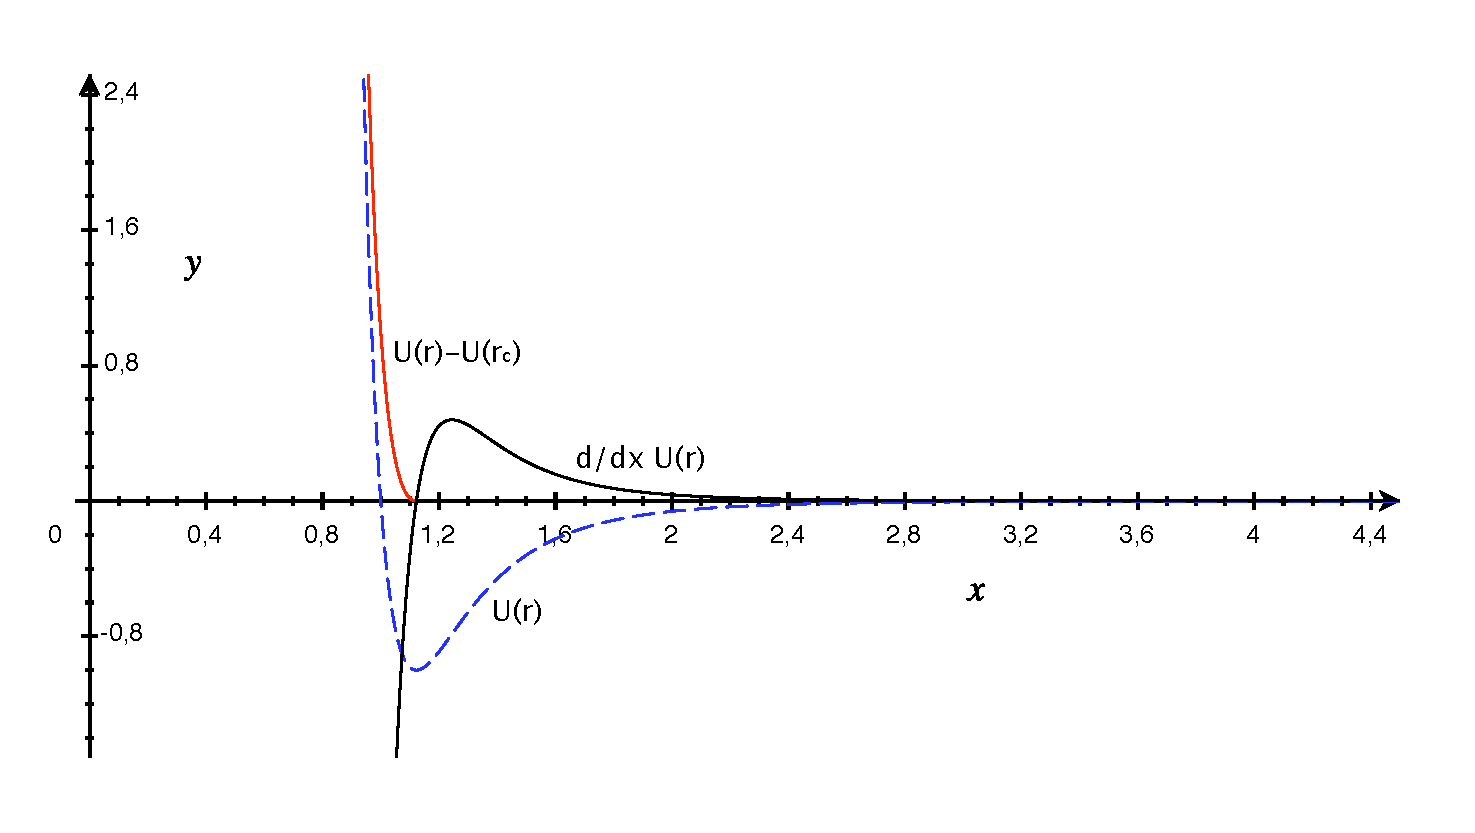
\includegraphics[width=12cm]{figures/lennard-jones-potential.pdf}
%\caption{Lennard Jones Potential - \newline ttt}
\caption[long text]{Lennard Jones Potential with
  $\epsilon=1$ and radius $\sigma=1$. If you use a large cutoff such as
  $2.5\sigma$, the potential is practically zero at the cutoff. The
  red curve indicates the Weeks-Chandler-Andersen potential, which
  is obtained from the Lennard-Jones potential by cutting it off in
  its minimum at $r_c=\sqrt[6]{2}$ and shifting it up.}
\label{pic:lennard-jones}
\end{center}
\end{figure}

\noindent 
The \lstinline|writepdb| command writes the atomic configuration in the PDB (Brookhaven Protein DataBase) format to the given file. This standard formatted file can easily be imported to standard applications like VMD. 

As it was said in \ref{sec:partprop} we had to set up the interactions between all groups separately. 
After we have set the necessary environment we must warmup our system before we run the simulation. We set 
particles at random positions so some particles can overlap. In this situation \es  will crash with an error:
particle out of range. To take particles apart 
we cap forces  by setting the Lennard-Jones force constant below a certain distance. 
Therefore we use the \lstinline|inter forcecap| command. We do the procedure  \verb"$warm_n_times" times 
for \verb"$warm_steps" steps and stop only if the minimal distance between particles is also larger than 
\verb"$min_dist", that was set earlier.  To turn 
the capping off, we set ljforcecap to 0. Then  we equilibrate our system until all relevant physical observables
are fluctuating around their mean values. In the case of Lennard Jones it is enough to monitor energy. 
To equilibrate we rescale particles' velocities to reach the target temperature.


{\small\vspace{0,2cm}
\begin{lstlisting}[firstnumber=auto]{bsp_code}
#############################################################
#  Warmup Integration                                       #
#############################################################

set act_min_dist [analyze mindist]
puts "Start with minimal distance $act_min_dist"

# open Observable file

puts "\nStart warmup integration:"
puts "At maximum $warm_n_times times $warm_steps steps"
puts "Stop if minimal distance is larger than $min_dist"

# set LJ cap
set cap 1.0
inter forcecap $cap

# Warmup Integration Loop, equilibrate particles
set i 0
while { $i < $warm_n_times && $act_min_dist < $min_dist } {
    integrate $warm_steps

    # Warmup criterion
    set act_min_dist [analyze mindist]
    puts -nonewline "run $i at time=[setmd time] (LJ cap=$cap) min dist = $act_min_dist\r"
    
     # to force the printout immediately and don't wait for the buffer been printed
    flush stdout

    # Increase LJ cap
    set cap [expr $cap+1.0]
    inter forcecap $cap
    incr i
}

inter forcecap 0

puts "\n Warm up finished \n"

### Thermalization 
setmd time_step $eq_tstep
for { set i 0 } { $i < $equilibration_iterations } { incr i } {
   integrate $equilibration_interval
   set energies [analyze energy]
   rescale_velocities  $target_temperature [setmd n_part]
   puts -nonewline "eq run $i at time=[setmd time] \r"
}

\end{lstlisting}}\vspace{0,2cm}

\noindent After we have set the necessary environment and warmed up our system, we can now start with the actual 
simulation. To analyse our data after the simulation, we open some files for writing the data in. 

{\small\vspace{0,2cm}
\begin{lstlisting}[firstnumber=auto]{bsp_code}
  puts "sampling "
setmd time_step $tstep

# files to save simulation data
set en [open "data/energy.dat" "w"]
set blockfile [open "data/sim_info.dat" "w"]

puts $en "#"
puts $en "#"
puts $en "#  Pressure    Kinetic    Potential  Temperature "
puts $en "# "
for {set i 0} { $i < $sampling_iterations } { incr i} {
     integrate $sampling_interval
     save_sim $blockfile "id pos v f q type" "all"
\end{lstlisting}}\vspace{0,2cm}

\vspace{1cm}
\framebox{\begin{minipage}{0.95\textwidth} 
   \begin{task}
   Study the file  \texttt{lj\_functions.tcl}, specifically the procedure 
   \texttt{save\_sim} and how it is called in \texttt{lj\_tutorial.tcl} file. 
   Then run \texttt{lj\_tutorial.tcl} and check \texttt{data} directory for the
   simulation data file. Inspect the simulation data file \texttt{sim\_info.dat}.
   
   Run \es{} by typing \texttt{Espresso lj\_tutorial.tcl} on the Linux command line.
   \end{task}

\end{minipage}}\vspace{1cm}

\noindent 
The  \lstinline|save_sim| statement calls the function defined in lj\_tutorial.tcl . We tell the function what parameters to be saved  and which particles we want to save (all).  Before continuing with our example we have a look at the \lstinline|save_sim| procedure

{\small\vspace{0,2cm}
\begin{lstlisting}[numbers=none]
proc save_sim {cfile parinfo range } {
 blockfile $cfile write variable all
 blockfile $cfile write tclvariable all
 blockfile $cfile write particles $parinfo $range
 blockfile $cfile write interactions
 blockfile $cfile write bonds
 blockfile $cfile write random
 blockfile $cfile write seed
}
\end{lstlisting}\vspace{0,2cm}
}
\noindent 
This procedure saves all variables available in our programme to \lstinline|$cfile| which is in our example sim\_info.dat. Have a look at the sim\_info.dat to see what that means

{\small\vspace{0,2cm}
\begin{verbatim}
{variable 
	{box_l 5.2387886 5.2387886 5.2387886}
	{cell_grid 2 2 2}
	{cell_size 2.6193943 2.6193943 2.6193943}
	{dpd_gamma 0.0}
	{dpd_r_cut 0.0}
	...
}
{tclvariable 
	{density 0.8442}
	{tstep 0.001}
	{energies { energy -384.41147 } { kinetic 121.41453 } { 0  0 nonbonded -505.826 }}
	{lj1_cut 2.5}
	{blockfile file6}
	...
}
{particles {id pos v f q type} 
	{0 13.08106 4.376436 2.4466876 1.2432192 ...}
	{1 -2.7657422 -0.09919841 -1.0362237 -0.4642931...}
	{2 4.4635587 5.4885591 5.460385 0.18670765 ...}
	{3 -2.9920063 0.88519503 7.3518191 0.5820964 ...}
	...
}
{interactions 
	{0 0 lennard-jones 1.0 1.0 2.5 0.0040792228 0.0 0.0 }
}
{bonds  
	{0 { } }
	{1 { } }
	...
}
{random 
	{1198928294 .... }
}
{seed 
	{16838}
}
...
\end{verbatim}
\vspace{0,2cm}
}
\noindent 
What do we see? We find that there are five types of blocks which are
repeated very often. The first block (variable) contains all \es{}
variables, the second (tclvariable) all variables of the tcl
script. In the third block we find the entire particle data we had
told the \lstinline|save_sim| function to save (id: particle id, pos:
position, v: velocity, : force, q: charge, type). \lstinline|save_sim|
saves interactions, bonds, random and seed.  In
our case the interaction is Lennard-Jones. The bonds block is empty
because the particles are not bound to each other like, for example,
in a polymer. The rest of the blocks contains information (random,
seed) to be able to restore the status of the
random generator as it was while writing these blocks.  What do we
need that for? If we rerun the simulation we will get the same results
after we have set our variables including the random generator
status. Looking at the example script, we see that the
\lstinline|save_sim| function is called every time in the loop; that
is why the blocks are repeated.

\vspace{1cm}\framebox{\begin{minipage}{0.95\textwidth} 
   \begin{task}
    
    Study and run \texttt{blockfile\_read.tcl}  to see how to read offline 
    data. Modify this script to print out simulation time and average particle
    positions $x_{avg},y_{avg},z_{avg}$.
    
   \end{task}

\end{minipage}}\vspace{1cm}
%\marginpar{Sample solution}

In the energy.dat file we print out the values for pressure, kinetic
and potential energies, temperature obtained with the command
\lstinline|analyze| \texttt{energy}.


{\small\vspace{0,2cm}
\begin{lstlisting}[firstnumber=auto]{bsp_code}
     set energies [analyze energy]
     set pressure [analyze pressure total]
     set total [expr [lindex $energies 0 1]/$n_part]
     set kinetic [expr [lindex $energies 1 1]/$n_part]
     set potential [expr [lindex $energies 2 3]/$n_part]
     set kinetic_temperature [expr [lindex $energies 1 1]/(1.5*[setmd n_part])]
     set temperature $kinetic_temperature
     puts $en "$i   $pressure  $kinetic  $potential  $temperature $total"
     lappend apressure $pressure
     lappend akinetic $kinetic
     lappend apotential $potential
     lappend atemperature $temperature
     lappend atotal $total
     puts -nonewline "integration step   $i / $sampling_iterations \r"
}
close $en
\end{lstlisting}}\vspace{0,2cm}

\noindent \texttt{kinetic temperature} here refers to the measured temperature obtained from kinetic energy and
the number of degrees of freedom in the system. It should fluctuate around the preset temperature of the thermostat.

\newpage
\vspace{1cm}\framebox{\begin{minipage}{0.95\textwidth} 
    \begin{task}
      Plot the time evolution of pressure and energy, which are written into the
      \texttt{data} directory in the file \texttt{energy.dat}.
    \end{task}
  \end{minipage}}\vspace{1cm}

The result plot for \texttt{energy.dat}
should be similar to this one:
\begin{center}
  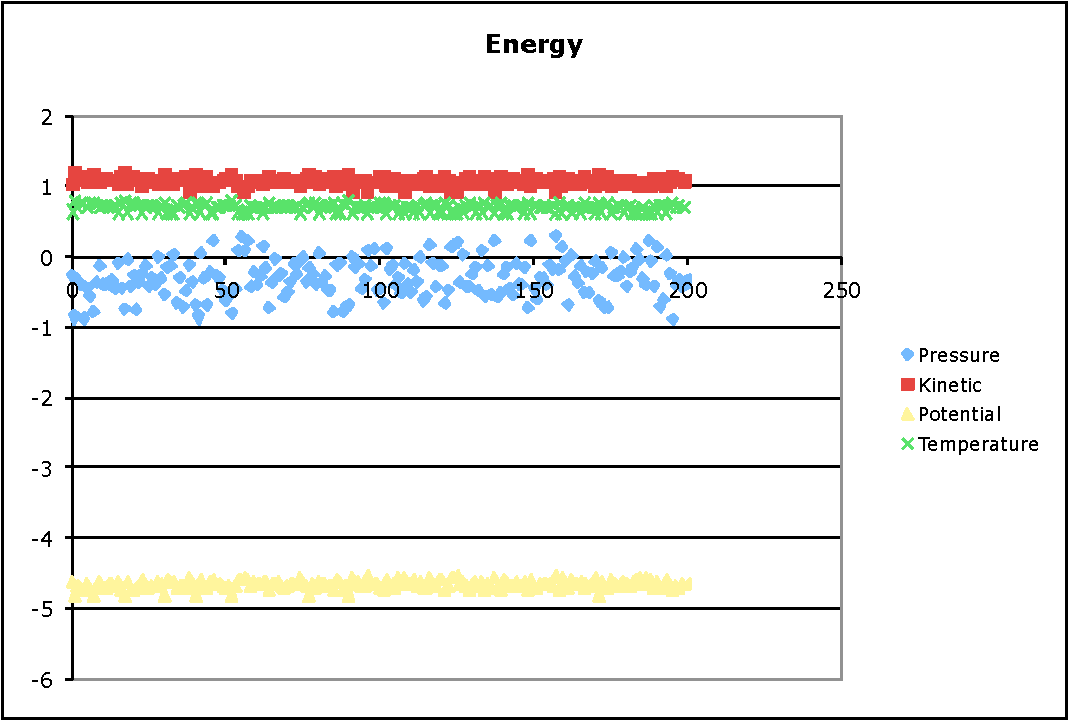
\includegraphics[width=10cm]{figures/energy}
\end{center}
\noindent As we can see the system is in equilibrium because pressure, potential and kinetic energy per particle 
and calculated current temperature fluctuate around their mean values.

%%%%%%%%%%%%%%%%%%%%%%%%%%%%%%%%%%%%%%%%%%%%%%%%%%%  
   





%\subsection{Data visualization}\label{sec:vmd}
   
%   \marginpar{Add detailed results to this section, so that the tutorial can
 %  also be done without the aid of an expert.}
   
\subsection{Simple Error Analysis on Time Series Data with \texttt{uwerr}}

  \noindent Espresso provides a build-in time series analysis tool called \lstinline|uwerr|.
  In our simulation we don't know if values of the same variable that we got from two adjacent samples are
  correlated or not and sampling too seldom will lead either to long runs of the simulation
  or to bad statistics. On the other hand, sampling too often leads to strong correlations between the samples,
  which will make us underestimate the statistical errors in our measurements using usual formulas e.~g.
  for the standard deviation.
  \lstinline|uwerr| is used to determine the mean and its standard 
  error  of total energy per particle for arbitrary numerical time series based on
  the article by Wolff \cite{wolff}. Unlike the standard formulas, it can be used even with strongly correlated samples.

  Here to obtain, for example, the error for the total energy we submit as a first argument for 
  \lstinline|uwerr| the array of all measured values of total energy   \verb"$atotal", and then the total
  number of samples   \verb"$sampling_iterations". 1 as the third argument means that we ran only
  one full measurement (complete simulation). In general, the mean value could be also obtained
  from several simulations, providing  \verb"$atotal" then as a matrix, not as an array, the total
  number of samples for every simulation should be the same and the third argument for \lstinline|uwerr|
  would be the number of simulations. \lstinline|uwerr| returns a string, the first value of which is 
  a calculated mean value and the second is its error.

{\small\vspace{0,2cm}
\begin{lstlisting}[firstnumber=auto]{bsp_code}
  puts "--Reporting Energies and Temperature"
  set error [uwerr $atotal $sampling_iterations 1 ]
  set value [lindex $error 0]
  set verror [lindex $error 1]
  puts "     Total Energy: $value  $verror"
  set error [uwerr $akinetic $sampling_iterations 1 ]
  set value [lindex $error 0]
  set verror [lindex $error 1]
  puts "     Kinetic Energy: $value  $verror"
  set error [uwerr $apotential $sampling_iterations 1 ]
  set value [lindex $error 0]
  set verror [lindex $error 1]
  puts "     Potential Energy: $value  $verror"
  set error [uwerr $atemperature $sampling_iterations 1 ]
  set value [lindex $error 0]
  set verror [lindex $error 1]
  puts "     Temperature : $value  $verror"
  set error [uwerr $apressure $sampling_iterations 1 ]
  set value [lindex $error 0]
  set verror [lindex $error 1]
  puts "     Pressure : $value  $verror"
exit
\end{lstlisting}}%\vspace{0,2cm}
\noindent The last line here is the last line of the script terminating the process.

%\vspace{1cm}\framebox{\begin{minipage}{0.95\textwidth} 
%     \begin{task}
      
%      Inspect what \texttt{analyze energy} command returns. Make the similar 
%      error analysis for kinetic  temperature, kinetic energy and potential 
%      energy, in the main script.
%     \end{task}

%\end{minipage}}\vspace{1cm}


\vspace{1cm}\framebox{\begin{minipage}{0.95\textwidth} 
     \begin{task}
           
     Inspect what \texttt{analyze pressure total} command returns. Make a 
     similar error analysis for total pressure.
     \end{task}

\end{minipage}}\vspace{1cm}

\noindent \textbf{Hint:} \texttt{analyze pressure} (without \texttt{total}) returns the pressure and
corresponding contributions to it.
\newpage

\subsection{Online analysis of correlations}
\label{subsection:online_analysis}
\es{} can do online analysis of observables and correlations. This means that part of the analysis
is run on the fly during the simulation without first writing the configuration data to disk and re-reading it later on for analysis.
 To illustrate this the script calculates the mean square displacement of the particles online. 
The mean square displacement (MSD) is the average squared distance that a particle traveled during a given time.
It is defined by

$$
\text{MSD}(t) = \langle \Delta r(t) ^{2} \rangle = \frac {1} {N} \sum_{i=0}^{N} | r_{i}(t)-r_{i}(0) | ^{2}
$$

See section \ref{subsection:other_useful_scripts} for an offline version of the MSD calculation. The basic idea is to have a set of observables
that can be evaluated and correlated as needed. In the script the correlation for the mean square displacement of the particle is setup by

{\small\vspace{0,2cm}
\begin{lstlisting}[numbers=none]
# Setup observable for the positions
set obs_pos [observable new particle_positions all]
# Setup msd as position correlation
set msd [correlation new obs1 $obs_pos corr_operation square_distance_componentwise dt $tstep tau_max [expr 50.*$tstep]]
\end{lstlisting}\vspace{0,2cm}
} 

First a new observable is created via the \texttt{observable new} command, which is then used to create a new correlation. Here we use the predefined observable \texttt{particle\_positions}. There is a large set of predefined obsevables which are listed in the users guide. Observables can also defined as TCL functions provided by the user, please refer to the documentation.
 
The \texttt{correlation} command can create arbitraty time-correlations between observables. In this case
we want to calculate the position auto correlation. Autocorrelations are created by only passing one observable to the command. The most important other parameters are the \texttt{corr\_operation}, which is the operation performed by bevor averaging, here the observable is squared componentwise. For a list of predefined operations please have a look at the documentation. The maximum timespan for which the correlation function should be sampled is set by \texttt{tau\_max}.

Observables can either be updated automatically in regular intervals or explicitly by the user. In the script we update explicitly by calling

{\small\vspace{0,2cm}
\begin{lstlisting}[numbers=none]
correlation $msd update
\end{lstlisting}\vspace{0,2cm}
} 

Finally after the sampling phase we have to write the calculated MSD to the disk.
Since we calculated the correlation separately for every component of every particle we first
average over all the components to improve statistics.

{\small\vspace{0,2cm}
\begin{lstlisting}[numbers=none]
# Get calculated MSD from correlator
set msd_data [correlation $msd print]
# Open file to write MSD to
set msd_file [open "data/msd_correlator.dat" "w"]

# Loop over all the times
foreach msd_sample $msd_data {
    # Holds the average over all the components of all the particles
    set average 0.0
    # Current time
    set tau [lindex $msd_sample 0]
    # Loop over all the components of all the particles for this time
    for { set i 0 }  { $i < [expr 3*$n_part] } { incr i } {
        # and sum them up
	set average [expr $average + [lindex $msd_sample [expr $i + 2]]]
    }
    # Normalize
    set average [expr $average/(3*$n_part)]
    # Write to file
    puts $msd_file "$tau $average"
}

close $msd_file
\end{lstlisting}\vspace{0,2cm}
} 


\es{} employs an algorithm called \emph{multiple $\tau$ correlator} to calculate the correlation function
that makes it efficient to calculate correlations for very long times (cf. \cite{frenkel02b}), possibly over the run of the complete
simulation. The correlator is a very powerful tool that is very flexible and can do many types of calculations.
An in-depth discussion of its features would be a tutorial in its own right and is beyond the scope of this
one, but it might be worthwhile to read up on it and see if it can solve your problem before you implement
something yourself. The predefined observables and correlation functions are implemented in the \es{} core and
are typically several orders of magnitude faster than analysis that is implemented on the TCL level.

\vspace{1cm}\framebox{\begin{minipage}{0.95\textwidth} 
     \begin{task}  
      Inspect the code for the MSD calculation and plot the MSD from \texttt{data/msd\_correlator.dat}. 
      Try different parameters  for the \texttt{correlator} command, such as the sample length and the number of points. 
      What do you observe if you make the maximal tau bigger? Can you find out how to calculate the velocity autocorrelation instead?
     \end{task}
\end{minipage}}\vspace{1cm}

\subsection{Other Useful Scripts}
\label{subsection:other_useful_scripts}
The radial distribution function (RDF) describes the distribution of particles around
the center of a fixed particle, as a function of the particle-particle distance. This of course assumes
that the particle distribution is isotropic around the particles.

\vspace{1cm}\framebox{\begin{minipage}{0.95\textwidth} 
     \begin{task}  
      Run \texttt{rdf.tcl}, inspect the 
      code and plot the RDF from \texttt{data/rdf.dat}. Try different parameters 
      for the \texttt{analyze rdf} command, such as the bin size. What do you observe?
     \end{task}

\end{minipage}}\vspace{1cm}

\begin{figure}[ht]
\begin{center}
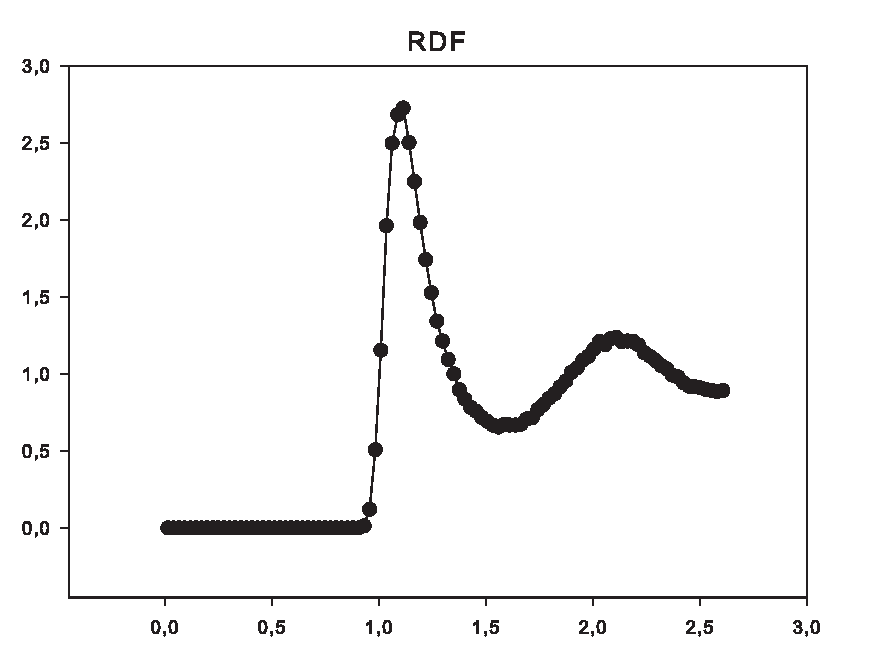
\includegraphics[width=10cm]{figures/rdf}
\label{fig:rdf}
\caption{The rdf.dat plot should be similar to this one}
\end{center}
\end{figure}

\noindent Our RDF is structureless, which means we have liquid. If the bin size is increased, the number of points in the
graph will also increase, but due to poorer sampling the curve will not be smooth anymore. 

\newpage

The velocity autocorrelation function (VACF) is an averaged time dependent correlation function of all particles' 
velocities. 

\vspace{1cm}\framebox{\begin{minipage}{0.95\textwidth} 
     \begin{task}  
      Run \texttt{vacf.tcl}, inspect 
      the code and plot the VACF from \texttt{data/vacf.dat}. The VACF $C(t)$ can 
      be computed directly: \[ C(t) = \langle \mathbf{v}_{i} (0) \mathbf{v}_{i} 
      (t) \rangle \] which can be estimated by \[ C(t) = \frac {1} {N} \sum_{i=0}^{N} \mathbf{v}_{i} (0) 
      \mathbf{v}_{i} (t) \] where $N$ is the number of particles.
        
        Try to modify \texttt{vacf.tcl} by using \texttt{vecsub} and 
        \texttt{veclen} and the tcl math functions.
     \end{task}

\end{minipage}}
\vspace{1cm}
%\marginpar{Script anpassen, sodass kleineres dt, um bessere Aufl\"osung zwischen 0...50 zu erhalten}

\begin{figure}[ht]
\begin{center}
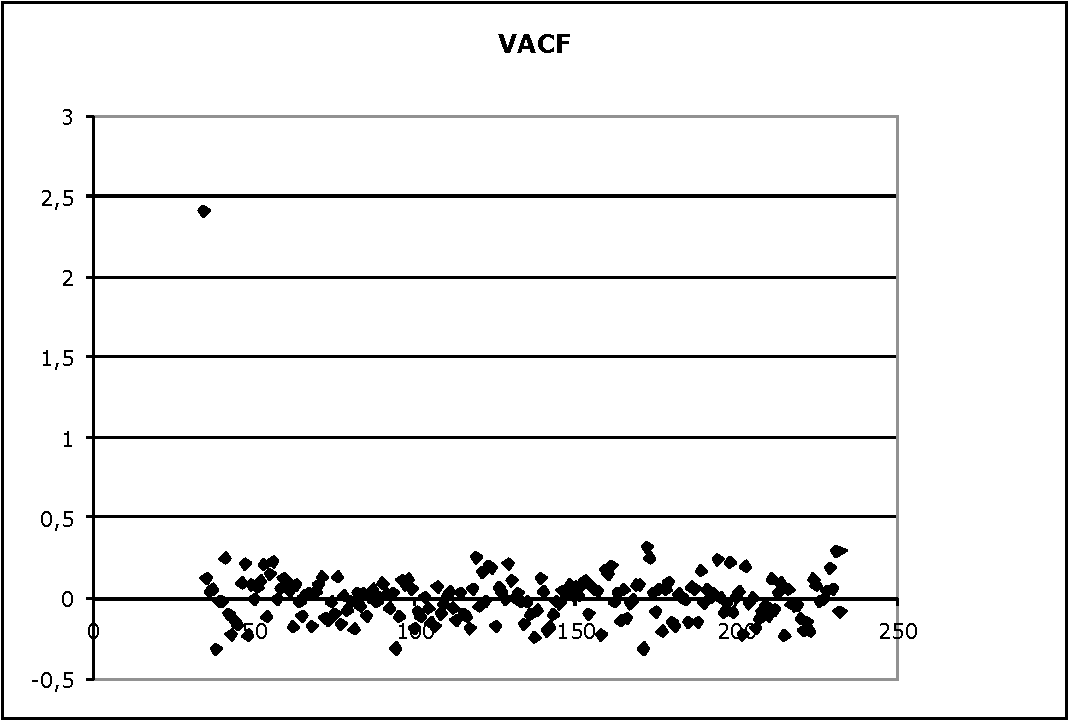
\includegraphics[width=10cm]{figures/vacf}
\label{fig:vacf}
\caption{The vacf.dat plot should be similar to this one}
\end{center}
\end{figure}

\noindent We can see when time is bigger than 50 the particles have already 'forgot' about their initial
velocities. Sampling more in the time interval [0;50] will show the decay of VACF there.

\newpage

We can also calculate the mean square displacement (MSD) from the offline data (see section \ref{subsection:online_analysis} for an online version of the calculation).
The mean square displacement (MSD) is the average squared distance that a particle traveled during a given time.

\vspace{1cm}\framebox{\begin{minipage}{0.95\textwidth} 
     \begin{task}  
      Run \texttt{msd.tcl}, inspect the code 
      and plot the MSD from \texttt{data/msd.dat}. The MSD can be simply computed 
      by: \[ \langle \Delta r(t) ^{2} \rangle  = \frac {1} {N} \sum_{i=0}^{N} 
      \Delta \mathbf{r}_{i}(t)^{2} \] or \[ \langle \Delta r(t) ^{2} \rangle = 
      \frac {1} {N} \sum_{i=0}^{N} | r_{i}(t)-r_{i}(0) | ^{2} \]
     \end{task}

\end{minipage}}
\vspace{1cm}

\begin{figure}[ht]
\begin{center}
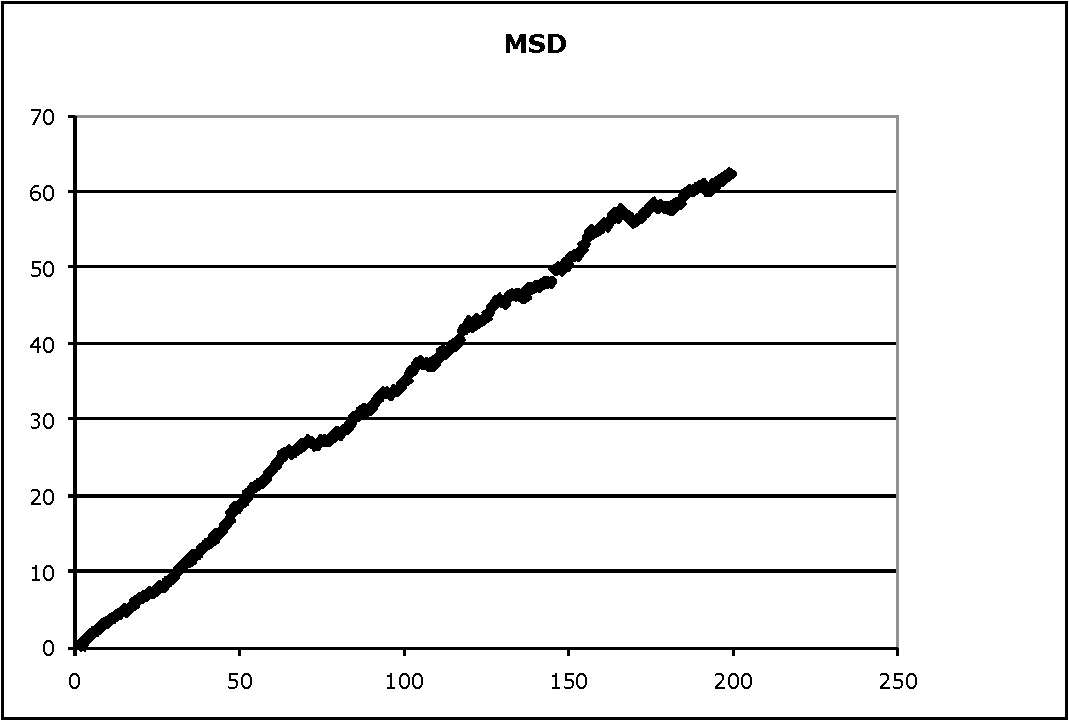
\includegraphics[width=10cm]{figures/msd}
\label{ }
\caption{The msd.dat plot should be similar to this one}
\end{center}
\end{figure}

\noindent On short time scales a particle does not collide with others
(ballistic regime) so the distance traveled should be proportional to
the time and therefore the MSD should increase quadratically. On
bigger time scales, a particle performs sort of a random walk due to
many interactions with other particles. This regime is called
diffusive; in this regime the MSD increases linearly with time. The coefficient of
proportionality is the diffusion coefficient: $D=\frac{1}{2 d t} \langle
\Delta r(t) \rangle^2$, where d is the dimensionality of the problem and $t$ the
traveling time.

If \texttt{msd.dat} is plotted in log-log scale, then ballistic and diffusive regimes will be visible even better
(better sampling won't harm).

\bibliographystyle{unsrt}
\bibliography{refs}
\end{document}

